\documentclass[14pt, a4paper]{book}
\usepackage[utf8]{inputenc}
\usepackage[T1]{fontenc}
\usepackage[margin=1in]{geometry} 
\usepackage{amsmath,amsthm,amssymb,amsfonts, fancyhdr, color, comment, graphicx, environ, bm}
%\usepackage{xcolor}
%\usepackage{mdframed}
\usepackage[shortlabels]{enumitem}
\usepackage[american]{duomasterforside}
%\usepackage{indentfirst}
%\usepackage{simpler-wick}
\usepackage{booktabs}
%\usepackage{siunitx}
\usepackage{physics}
%\usepackage{polynom}
%\usepackage{verbatim}
%\usepackage{tensor}
\usepackage{todonotes}
%\usepackage{dcolumn}% Align table columns on decimal point
\usepackage{listings}
\usepackage{caption}
\usepackage{subcaption}
\usepackage[backend = biber, style = vancouver]{biblatex}
\bibliography{refs.bib}
\usepackage{hyperref}
\hypersetup{
    colorlinks=true,
    linkcolor=blue,
    filecolor=magenta,      
    urlcolor=cyan,
    citecolor=cyan,
    %pdftitle={Overleaf Example},
    %pdfpagemode=FullScreen,
    }

\newcommand\signature[2]{% Name; Department
\noindent\begin{minipage}{5cm}
    \noindent\vspace{3cm}\par
    \noindent\rule{5cm}{1pt}\par
    \noindent#1\par
    \noindent\textit{#2}%
\end{minipage}}
\newcommand\insertdate[1][\today]{\begin{flushright}#1\end{flushright}}


\title{Model independent search for Dark Matter
% }\subtitle{
in dilepton + MET final states with the ATLAS detector at the LHC 
}
\author{Ruben Guevara}
\date{Spring 2023}

\begin{document}
\pagenumbering{roman}
\duoforside[
dept = {Department of Physics},
long,
program = {Physics: Nuclear and Particle Physics},
]
\newpage
\section*{Acknowledgements}
Thank you everybody<3<3

\newpage
\begin{center}
\section*{Abstract}
Something something
\end{center}


\newpage
\tableofcontents
\listoffigures
\listoftables

\newpage
\pagenumbering{arabic}
\part{The theory behind modern particle physics}


\chapter{The Standard Model of Particle Physics and Beyond}

\section{The Basics}
\subsection{Classical Field Theory}


\subsection{Quantum Mechanics}


\subsection{Special Relativity}


\section{Quantum Field Theory}


\subsection{Fermionic and Bosonic fields}


\subsection{Quantum Electro Dynamics}

\subsection{Quantum Chromo Dynamics}


\subsection{Electroweak unification}


\subsection{The Brout-Englert-Higgs Mechanism}


\subsection{The Standard Model of Particle Physics}


\section{Beyond Standard Model}

\subsection{Dark Matter}



\chapter{Detection and Analysis}


\section{The ATLAS Detector}


\section{Classical Data Analysis}



\chapter{Machine Learning}


\section{Neural Networks}
Since the goal is to use ML to get a high accuracy to distinguish signal from background we have to start from the ML basics.  This project will take from granted that the reader is comfortable with linear algebra and jump straight into ML. The essence of machine learning is to use cost functions to tweak some parameters until it gives satisfactory predictions for the task given. In this project we will do Supervised Learning (meaning we know what the output should be) and only look at Neural Networks (NN) as our ML algorithm, since the ultimate goal is to "upgrade" this to run it on a quantum computer. The parameters mentioned above are called \textit{weights} and \textit{biases} for NNs. Considering a general parameter $\bm{\beta} = \{\beta_1,\beta_2,\cdots,\beta_n\}$ for a n-dimensional problem, the goal is to choose these parameters $\bm{\beta}$ such that we minimize a cost function $C(\bm{\beta})$ with respect to a set of data points given by a matrix $\mathbf{X}$, which in the case of the HiggsML are the features. And target values $\mathbf{t}$, which on the HiggsML are the labels. Before we get into that we can start by looking at Stochastic Gradient Descent (SDG).

\subsection{Stochastic Gradient Descent}
Before explaining the SDG we have to look at the Regular GD. Given a cost function $C(\bm{\beta})$ we can get closer to the minimum by calculating the gradient $\nabla_{\beta}C(\bm{\beta})$ wrt. the unknown parameters from the NN $\bm\beta$. If we were to calculate the gradient at a specific point $\bm{\beta}_i$ in the parameter space, the negative gradient would correspond to the direction where a small change $d\bm\beta$ in the parameter space would result in the biggest decrease in the cost function. In the same way we in physics would determine where the local (or global) minima at a complex multidimensional potential numerically. In GD we can chose a step size $\eta$ to choose how much we want to iterate in the parameter space, this is called the \textit{learning rate}. The mathematical function for an iteration to choose the parameter $\bm{\beta}$ such that it decreases the cost function is given as
\begin{equation}\label{eq:GD}
    \bm{\beta}_{i+1}=\bm{\beta}_{i} -\eta\nabla_{\beta}C(\bm{\beta}_i)
\end{equation}
To converge towards a minimum we should choose a learning rate $\eta$ small enough to not "step over" the minimum point of the cost-function-space. One thing to note here is that we could get trapped on a local minima rather than the global minima which is the ultimate goal. So choosing the learning rate as a hyperparameter to be changed in a grid search is a good way to find the best one.\\
\\In GD one computes the cost function and its gradient for all data points together. This quickly becomes computationally heavy when dealing with large datasets. Thus a common approach is to compute the gradient over batches of the data. For example in the HiggsML, instead of making a $30\times250,000$ matrix we could rather split it into smaller batches of maybe $30\times1,000$ to then perform a parameter update, making the computation faster. This is where SGD comes in, for each step, or epoch the data is divided randomly into \textit{N} batches of size \textit{n}. Then for each batch we use Eq. (\ref{eq:GD}) to update the parameters, thus updating $\bm{\beta}_{i+1}$ \textit{N}-times for each epoch. The idea of SGD comes from the observation that the cost function can almost always be written as a sum over \textit{n} data points. As mentioned above the main advantage of SGD is the computation time, but it also reduce the risk of getting stuck in a local minima since it introduces a randomness of which part of the parameter space we move through.

\subsection{Artificial neurons}
As stated by Hjorth-Jensen in \cite{MORTYY1}:
\begin{quote}
    \textit{The idea of NN is to to mimic the neural networks in the human brain, which is composed of billions of neurons that communicate with each other by sending electrical signals. Each neuron accumulates its incoming signals, which must exceed an activation threshold to yield and output. If the threshold is not overcome, the neuron remains inactive, i.e. has zero output}
\end{quote}
To describe the behaviour of a neuron mathematically we can use the following model
\begin{equation}\label{eq:neurons}
    y=f\left(\sum_{i=1}^{n}w_ix_i\right)=f(u)
\end{equation}
Where $y$, the output of the neuron, is the value of its \textit{activation function}, which has the weighted ($w_i$) sum of signals $x_i,\cdots,x_n$ received by $n$ neurons.\\
\\Since the goal of NNs is to mimic the biological nervous system by letting each neuron interact with each other by sending signals, which for us is of the form of a mathematical function between each layer. Most NNs consist of an input layer, an output layer and maybe layers in-between, called hidden layers. All the layers can contain an arbitrary number of neurons, and each connection between two neurons is associated with a weight variable $w_i$. The goal of using NNs is to teach the network the patterns of the data to then predict something. In the context of the HiggML, by giving a NN our data as its input layer, we can then train the network to distinguish signal from background.\\ \\Explained in greater detail if we were to look at a single event of the data, we start with an input with all 30 features of the event. Using Eq. (\ref{eq:neurons}) on every neuron on the next layer we can teach the network if there is are any connections between the features, we can repeat this process for \textit{n} layers. As an output we want a single neuron to see if it has predicted the event to be a signal or background, since this is binary output. After seeing the prediction we can use the labels to tell the network whether it predicted correctly or wrong since we are doing Supervised Learning. We can then use a \textit{cost function} and a specific \textit{metric} to evaluate numerically how network the predicted the output with a score. Seeing how the results fare we can then back-propagate to shift the weights and biases and repeat the process until we are satisfied with our result. Each of these iterations is called an epoch.\\
\\To generalize our artificial neuron to a whole network we can look at a Multilayer Perceptron (MLP). An MLP is a network consisting of at least three layers of neurons, the input, one or more hidden layers, and an output. The number of neurons can vary for each layer. The above explanation is a very dense and simplified one. In reality it is complicated to find out which cost function, activation function, metric, etc. is best suited the problem. But before we get into the details we can explore the mathematical model that illustrates what was tried to be explained above. 


\subsection{Activation functions}
As seen above, an important aspect of NNs are activation functions and cost functions. As shall become apparent soon, when evaluating an activation function we get the neuron output, but what are these activation functions? Mathematically speaking, activation functions are: Non-constant, Bounded, Monotonically-increasing and continuous functions. For this project we utilize both a sigmoid activation function
\begin{equation}\label{eq:sig}
    f(x) = \frac{1}{1+e^{-x}}
\end{equation}
which is the most basic activation function. We also utilise a Rectified Linear Unit (ReLU)
\begin{equation}\label{eq:ReLU}
    f(x) = x^+ = \text{max}(0,x) = \begin{cases}x&{\text{if }}x>0,\\0.&{\text{otherwise}}.\end{cases}
\end{equation}
which has better gradient propagation, meaning that there are fewer vanishing gradient problems compared to the sigmoidial function.


\subsection{Cost functions}
Another aspect are cost functions. Cost functions are what we will utilize to evaluate how well the output of the network fares against the target, i.e. if our network "guesses" right whether a event is signal or background, thus making this a very important part of our network! Before getting into this we first have to look at logistic regression. For the HiggsML we will study a binary case where the output is either $t_i=0\vee 1$, meaning background or signal. We can introduce a polynomial model of order $n$ as
$$
\hat{y}_i=\beta_0+\beta_1x_i+\beta_2x_i^2+\cdots+\beta_nx_i^n
$$
where we then can define the probabilities of getting $t_i=0\vee1$ given our input $x_i$ and $\bm{\beta}$ with the help of a logistic function. Using the same sigmoid function as in Eq. (\ref{eq:sig}) as a logistic function, only calling it $p(t)$. We get the probability as
$$
p(t_i=1\vert x_i,\bm{\beta})=\frac{1}{1+e^{-\hat{y}_i}}
$$
and
$$
p(t_i=0\vert x_i,\bm{\beta})=1- p(y_i=1\vert x_i,\bm{\beta})
$$
We want to then define the total likelihood for all possible outcomes from a dataset $\mathcal{D}=\{(t_i,x_i)\}$, with the binary labels $t_i\in\{0,1\}$, to do this we use the Maximum Likelihood Estimation (MLE) principle. This gives us
$$
P(\mathcal{D}\vert\bm{\beta})=\prod_{i=1}^n\left[p(t_i=1\vert x_i,\bm{\beta})\right]^{t_i}\left[1-p(t_i=1\vert x_i,\bm{\beta})\right]^{1-t_i}
$$
from which we obtain the log-likelihood
$$
C(\bm{\beta})=\sum_{i=1}^n\left(t_i\log p(t_i=1\vert x_i,\bm{\beta})+(1-t_i)\log[1-p(t_i=1\vert x_i,\bm{\beta})]\right)
$$
By taking the parameter $\bm{\beta}$ to second order and reordering the logarithm we get
\begin{equation}\label{eq:CrossEntropy}
    C(\bm{\beta})=-\sum_{i=1}^n(y_i(\beta_0+\beta_1x_i)-\log(1+\exp(\beta_0+\beta_1x_i)))
\end{equation}
This equation is known as the \textit{cross entropy} which we will use in this project. The two beta parameters used are the weight and biases as will come apparent later.
The goal is to change these parameters such that it minimizes the cost function as we will see later. \\
\\Something else we will include in this project is to add an extra term to the cost function, proportional to the size of the weights. We do this to constrain the size of the weights, so they don't grow out of control, this is to reduce \textit{overfitting}. In this project we will use the so called \textit{L2-norm} where the cost function becomes
\begin{equation}\label{eq:reg}
    C(\bm\beta)=\frac{1}{N}\sum_{i=1}^N\mathcal{L}_i(\bm\beta)\rightarrow \frac{1}{N}\sum_{i=1}^N\mathcal{L}_i(\bm\beta)+\lambda\sum_{ij}w_{ij}^2
\end{equation}
Meaning we add a term where we sum up all the weights squared. The factor $\lambda$ is called the regularization parameter. The L2-norm combats overfitting by forcing the weights to be small, but not making them exactly zero. This is so that less significant features still have some influence over the final prediction, although small.


\subsection{Feed Forward network}
To describe how the network "guesses" outputs in a mathematical model we can compute we can start by looking at Eq. (\ref{eq:neurons}) where we got an output $y$ from an activation function $f$ that receives $x_i$ as input. We can expand the function as as following
\begin{equation}\label{eq:activation}
    y=f\left(\sum_{i=1}^nw_ix_i+b_i\right)=f(z)
\end{equation} 
where $w_i$ is still the weight and we introduced a bias $b_i$ which is normally needed in case of zero activation weights or inputs. The difference comes now in the interpretation where in the activation $z=(\sum_{i=1}^nw_ix_i+b_i)$ the inputs $x_i$ are the outputs of the neurons in the preceding layer. Furthermore an MLP is fully-connected, meaning that each neuron received a weighted sum of the output of \textbf{all} neurons in the previous layer. To expand Eq. (\ref{eq:activation}) we can first look at the output of every neuron $i$ in a weighted sum $z^1_i$ for each input $x_j$ on a layer
\begin{equation}\label{eq:weightedsum}
    z_i^1=\sum_{j=1}^Mw_{ij}^1x_j + b^1_i
\end{equation}
Such that if we evaluate the weighted sum in an activation function $f_i$ for each neuron $i$, then the output of all neurons in layer 1 is $y_i^1$
$$
    y^1_i=f(z_i^1)=f\left(\sum_{j=1}^Mw_{ij}^1x_j + b^1_i\right)
$$
Where \textit{M} stands for all possible inputs in a given neuron $i$ in the first layer, we have also assumed that we utilize the same activation function in the layer. To generalize this for $l$-layers, which may have different activation functions, we write it as
$$
    y^l_i=f^l(u_i^l)=f^l\left(\sum_{j=1}^{N_{l-1}}w_{ij}^ly^{l-1}_j + b^l_i\right)
$$
Where $N_l$ is the number of neurons in layer $l$. Thus when the output of all the nodes in the first hidden layer is computed, the values of the subsequent layer can be calculated and so forth until the output is obtained. With this we can show that we only need the the inputs $x_n$ to calculate the output with $l$ hidden layers
\begin{equation}\label{eq:MLP}
    y^{l+1}=f^{l+1}\left[\sum_{j=1}^{N_l}w^{l+1}_{ij}f^l\left(\sum_{k=1}^{N_{l-1}}w^{l}_{jk}\left(\cdots f^{1}\left(\sum_{n=1}^{N_0}w^1_{mn}x_n+b_m^1\right)\cdots\right)+b_j^{l}\right)+b^{l+1}_i   \right]
\end{equation}
This shows that an MLP is nothing more than an analytic function, specifically a mapping of real-valued vectors $\hat{x}\in\mathbb{R}^n\rightarrow\hat{y}\in\mathbb{R}^m$. We can also see that the above equation is essentially a nested sum of scaled activation functions of the form
$$
  f(x)=c_1f(c_2x+c_3)+c_4  
$$
where the parameters $c_i$ are the weight and biases. By adjusting these parameters we shift the activation function to better match the label we are training the data on, this is the flexibility of a NN. Something else we can note is that Eq. (\ref{eq:MLP}) can easily be changed into matrix notation, since this is trivial for high energy physicists I will spare myself the writing of matrix form on this project. However this realization can help make computing the values a much easier task by for example utilizing TensorFlow or other mathematical packages in Python. An illustration taken from \cite{MORTYY1} shows the main idea of how a Feed forward network is set up, this is shown in Figure \ref{fig:NN}.
\begin{figure}[!ht]
    \centering
    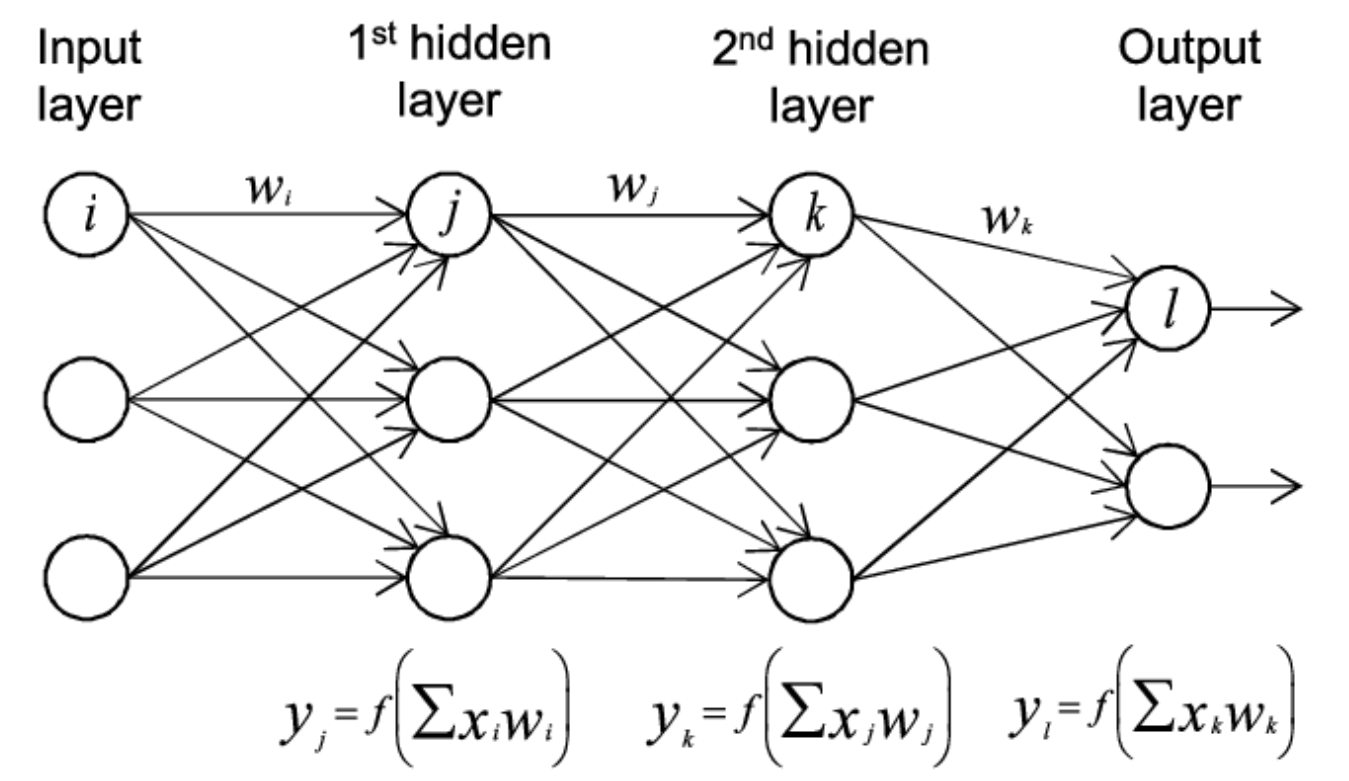
\includegraphics[width=0.5\linewidth]{NN.png}
    \caption[Basic Neural Network Illustration]{Basic illustration of a network with two hidden layers. Image taken from \cite{MORTYY1}}
    \label{fig:NN}
\end{figure}


\subsection{Back Propagation algorithm}
So far we have only explained Feed Forward networks, which helps us to compute the output of the NN in term of basic vector multiplications. It has also been mentioned that we can adjust the weight and biases, but never explained how. Now is the time to dive into that subject, as we will explain the back propagation algorithm. What we want to know is how do changes in the biases and the weights in the network change the cost function, and how we could use the final output to modify the weights? Before we derive these equations we an start by a plain regression problem and using the Mean Squared Error (MSE) as a cost function for pedagogical reasons
\begin{equation}\label{eq:cost}
    C(\hat{W})=\frac{1}{2}\sum_{i=1}^n(y_i-t_i)^2
\end{equation}
where $\hat{W}$ is the matrix containing all the weights and more importantly $t_i$ are our targets, which is in the HiggsML are the labels of events telling us whether we have a signal or background event. To generalise this we first have to go back to Eq. (\ref{eq:weightedsum}) generalize it for a layer $l$
$$
    z_i^l=\sum_{j=1}^Mw^l_{ij}y^{l-1}_j + b^l_i \Leftrightarrow \hat{z}^l=\left(\hat{W}^l\right)^T\hat{y}^{l-1} + \hat{b}^l
$$
where the right side is written on matrix notation. From the definition of $z_j^l$ with an activation function, i.e. Eq. (\ref{eq:activation}), we have
\begin{equation}\label{eq:partzw}
    \frac{\partial z_j^l}{\partial w_{ij}^l} = y_i^{l-1}
\end{equation}
and
$$
\frac{\partial z_j^l}{\partial y_i^{l-1}} = w_{ij}^l
$$
which again, with the definition of the activation function gives us
\begin{equation}\label{eq:partyz}
    \frac{\partial y^l_j}{\partial z_j^{l}} = y_j^l(1-a_j^l)=f(z_j^l)(1-f(z_j^l))
\end{equation}
We also need to take the derivative of Eq. (\ref{eq:cost}) with respect to the weights, doing so for a respective layer $l=L$ we have
$$
    \frac{\partial C(\hat W ^L) }{\partial w_{jk}^L}=\left(y_j^L-t_j\right)\frac{\partial y_j^L}{\partial w_{jk}^L}
$$
where the last partial derivative is easily computed using the chain rule with Eq. (\ref{eq:partzw}) and Eq. (\ref{eq:partyz})
$$
\frac{\partial y_j^L}{\partial w_{jk}^L} = \frac{\partial y^L_j}{\partial z_j^{L}}\frac{\partial z_j^l}{\partial w_{jk}^L} = y_j^L(1-y_j^L)y_k^{L-1}
$$
Such that we have
\begin{equation}\label{eq:CostW}
    \frac{\partial C(\hat W ^L) }{\partial w_{jk}^L}=\left(y_j^L-t_j\right)y_j^L(1-y_j^L)y_k^{L-1} :=\delta_j^Ly_k^{L-1}
\end{equation}
where we have defined the error
\begin{equation}\label{eq:delta}
    \delta_j^L:=\left(y_j^L-t_j\right)y_j^L(1-y_j^L)=f'(z_j^L)\frac{\partial C}{\partial y_j^L} 
\end{equation}
or in matrix form
$$
\delta^L = f'(\hat z ^L)\circ \frac{\partial C}{\partial \hat y ^L}
$$
where on the right hand side we wrote this as a Hadamard product. This error $\delta^L$ is an important expression, since as we can see on the index form of this expression on Eq. (\ref{eq:delta}), we can measure how fast the cost function is changing as a function of the $j$-th output activation. This means that if the cost function doesn't depend on a particular neuron $j$, then $\delta_j^L$ would be small.  \\
\\We also notice that everything in Eq. (\ref{eq:delta}) is easily computed. Thus we can also see how the weight changes the cost function using Eq. (\ref{eq:CostW}) quite easily. One thing else we can compute with Eq. (\ref{eq:delta}) is
$$
\delta_j^L=\frac{\partial C}{\partial z_j^L} =\frac{\partial C}{\partial y_j^L}\frac{\partial y_j^L}{\partial z_j^L}
$$
which can be interpreted in terms of the biases $b_j^L$
\begin{equation}\label{eq:bias}
    \delta_j^L=\frac{\partial C}{\partial b_j^L}\frac{\partial b_j^L}{\partial z_j^L} = \frac{\partial C}{\partial b_j^L} 
\end{equation}
where we see that the error $\delta_j^L$ is exactly equal to the rate of change of the cost function as a function of the bias.\\
\\Somerhing interesting as briefly mentioned above is that when using Eq. (\ref{eq:CostW} - \ref{eq:bias}) we see that if a neuron output $y_j^L$ is small, then the gradient term, Eq. (\ref{eq:CostW}), will also be small. We say then that the weight learns slowly, meaning that the contribution of said neuron is less important "to fix" than those that have a higher weight. Of course this example is a very simple one to wrap our heads around, but the magic comes when the algorithm is evaluating a random neuron in layer 20 on a deep learning algorithm, after so many layers it all becomes a \textbf{black box} for us to wrap our heads around!\\
\\It is also worth noting that when the activation function is flat at some specific values (depend on the chosen function) the derivative will tend towards zero making the gradient small meaning the network is learning slow as well. To finish up our back propagation algorithm we still need one more equation. We are now going to propagate backwards in order to determine the weight and biases. We start by representing the error in the layer before the final one $L-1$ in term of the errors of the output layer. If we try to express Eq. (\ref{eq:delta}) in terms of the output layer $l+1$. Using the chain rule and summing over all $k$ entries we get
$$
\delta_j^l=\sum_k\frac{\partial C}{\partial z_k^{l+1}}\frac{\partial z_k^{l+1}}{\partial z_j^l} =\sum_k \delta_k^{l+1}\frac{\partial z_k^{l+1}}{\partial z_j^l}
$$
recalling Eq. (\ref{eq:weightedsum}) (replacing $1$ with $l+1$) we get
\begin{equation}\label{eq:backprop}
    \delta_j^l=\sum_k\delta_k^{l+1}w_{kj}^{l+1}f'(z_j^l)
\end{equation}
Which is the final equation we needed to start back propagating. 

\subsection{Summary of idea}
To summarize the whole process of the NN
\begin{itemize}
    \item First take the input data $\mathbf{x}$ and the activation $\mathbf{z}_1$ of the input later, and then compute the activation function $f(z)$ to get the next neuron outputs $\mathbf{y}^1$. Mathematically this is taking the first step of the feed forward algorithm, i.e. choosing $l=0$ on Eq. (\ref{eq:MLP})
    \item Secondly we commit all the way on Eq. (\ref{eq:MLP}) and compute all $\mathbf{z}_l$, activation function and $\mathbf{y}^l$.
    \item After that we compute the output error $\bm{\delta}^L$ by using Eq. (\ref{eq:delta}) for all values $j$.
    \item Then we back propagate the error for each $l=L-1,l-2,\cdots,2$ with Eq. (\ref{eq:backprop}).
    \item The last step is then to update the weights and biases using Eq. (\ref{eq:GD}) for each $l$ and updating using
    $$
    w_{jk}^l\leftarrow w_{jk}^l-\eta\delta_j^ly_k^{l-1}
    $$
    and
    $$
    b_j^l \leftarrow b_j^l-\eta\delta_j^l
    $$
\end{itemize}
This whole procedure is usually called an epoch, which we can repeat as many times as we want to better reduce the cost function in hopes of getting to the global minima.

\section{Boosted Decision Trees}


\section{Ensemble modeling?}

\part{Implementation}
\chapter{Data Analysis}
\section{Background Estimation}
\section{Kinematic Variables}
\section{Dark Matter samples}

\chapter{Machine Learning}
\section{Data Preparation/LOG}
We are dropping $\Delta\Phi(l_1,l_2)$ and $\Delta\Phi(l_c,E_T^{miss})$ due poor overenstemmelse with data. The first one is most likely due us not including fake leptons (and also for all non SFOS final states). The latter is a problem that PhD. Even is being haunted by. There is also the problem of missing variables. For the dataset being used I only look at, at least, two jets in the final state. This does however not always happen, to "fill the gaps" I made the $p_T$ of the jets equal to zero if there are less than two events, which is physically reasonable. And more problematic, I set the $\eta$ and $\phi$ to 10, which has no physical meaning. Luckily this does not seem to be an important feature when training the network using XGBoost. There is also another problem, albeit less problematic than the previous ones, with the final states that are not SFOS, as the background on these tend to be lower than the data. The number of events that are not SFOS are minimal though, and we think the reason it doesn't fit the data is because we are not including fake leptons.

\subsection{Full Dark Matter dataset}
To train the networks I will utilize two methods. The first one being this where the dataset being sent into the ML network will contain every single DM MC sample available. So far there are 154 different MC samples, these are based on three theories. A Light Vector(LV), Dark Higgs (DH) and Effective Field Theory (EFT) vertex/propagator which produces the WIMP DM particles. As well as a new theoretical particle, $Z'$, and decays into the lepton pair observed. The three theories are divided further into MC samples with a Light Dark Sector (LDS) and High Dark Sector (HDS) which tells us the \todo{is this true?}range of the Dark Matter candidate mass. And lastly it is divided further into more MC samples with different masses for $Z'$. This dataset includes all of these samples such that the network learns Dark Matter in a model independent way.

\subsection{"Ensemble" dataset}
Another approach is to make multiple datasets and combine the results of every network into a "big network". This is the second approach which I call ensemble modelling. The thought behind this is that when teaching a network using the full dataset it might only focus on a few special ones that stand out more than others on the massive dataset. Also, every different DM sample has different phenomenology, specially in the future when I will be receiving SUSY samples, meaning that it also won't teach the network physics. Thus if we were to train a network one one sample at a time it would be the perfect scenario. However as will become apparent in Section \ref{sec:wgts}, the datasets (even the full DM dataset) are extremely unbalanced. To put some numbers, on each DM MC sample there are roughly 40,000 MC events, and for the SM background (with a massive MET > 50GeV cut!) there are roughly 87,000,000 MC events. Factoring the weights (i.e. cross sections) gives us an extremely low statistics dataset, even in the full DM dataset. \\
\\Thus making the approach to teach the networks one MC sample at a time is impossible \todo{for NN}. So far I have tried dividing the the MC samples into 18 different categories. First into their respective theory. Then into LDS or HDS. Then into three $m_{Z'}$ regions, where I've defined the \textit{low mass region} to be $\le 600$ GeV, the \textit{middle mass region} to be $>600 \cap\le 1100$ GeV and the\textit{ high mass region }to be $\ge 1100$ GeV. Using a NN with three hidden layers I get poor results, but changing this into one works! Will repeat with real weights, it didn't work. Will try DSID now...

\section{Neural Network Training}
\subsection{Weights}\label{sec:wgts}
The results so far (my \textit{OLD} interpretation with only three different DM theories) show that the network is completely capable of distinguishing signal from background in the unweighted training, however if we were to scale the predictions (the networks output) with the weights (sample weights * luminosity / sum of weights) we would see that the signal is hidden underneath the background. Both validation plots are shown in Figure \ref{fig:OLD_FULL_DM_VAL}. If we train the network using the weights of the MC samples we see that the network still gets the same accuracy, and an even lower loss function score. But the AUC becomes exactly 0.5. When looking at the ROC curve and validation plots (plots showing how well the network sorts signal from background) we see that everything "is messed up" the ROC is 0.5, and there is only \textbf{one} background bin. When printing how many signal events the weighted network predicted it is easy to understand why, it is because it says there is not a single dark matter event. Which I first interpreted as being in agreement with Figure \ref{fig:OLD_W_FULL_DM_VAL}.\\
\begin{figure}[!ht]
	\centering
	\begin{subfigure}[b]{0.8\textwidth}
        \centering
        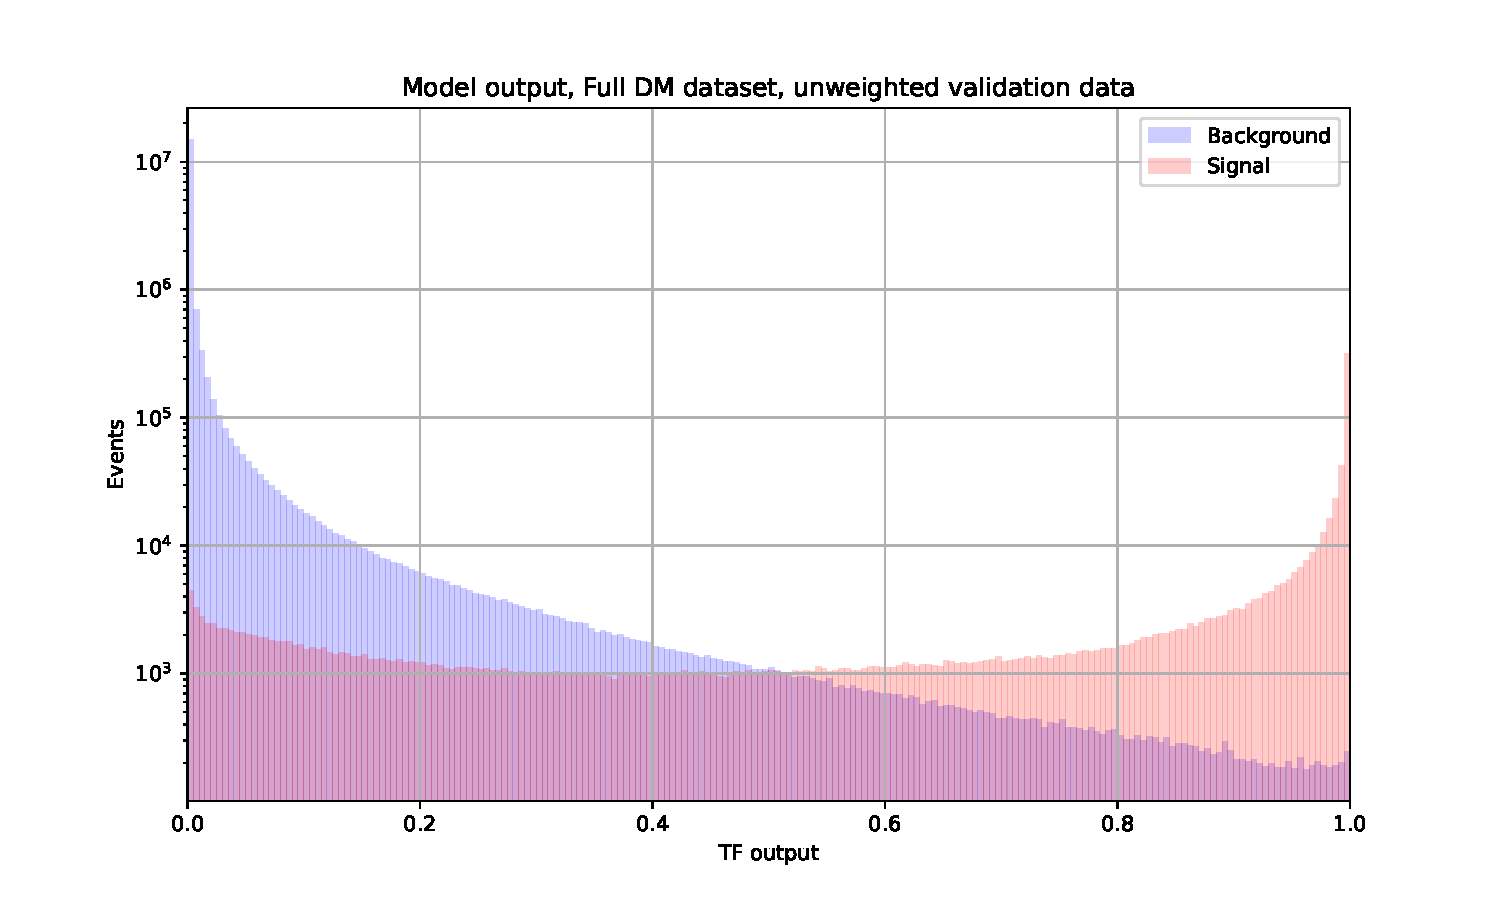
\includegraphics[width=1\textwidth]{OLD_DM_FULL_VAL_UNW.pdf}
        \caption{Unscaled validation plot.}\label{fig:OLD_UNW_FULL_DM_VAL}
     \end{subfigure}
     \hfill
     \begin{subfigure}[b]{0.8\textwidth}
        \centering
        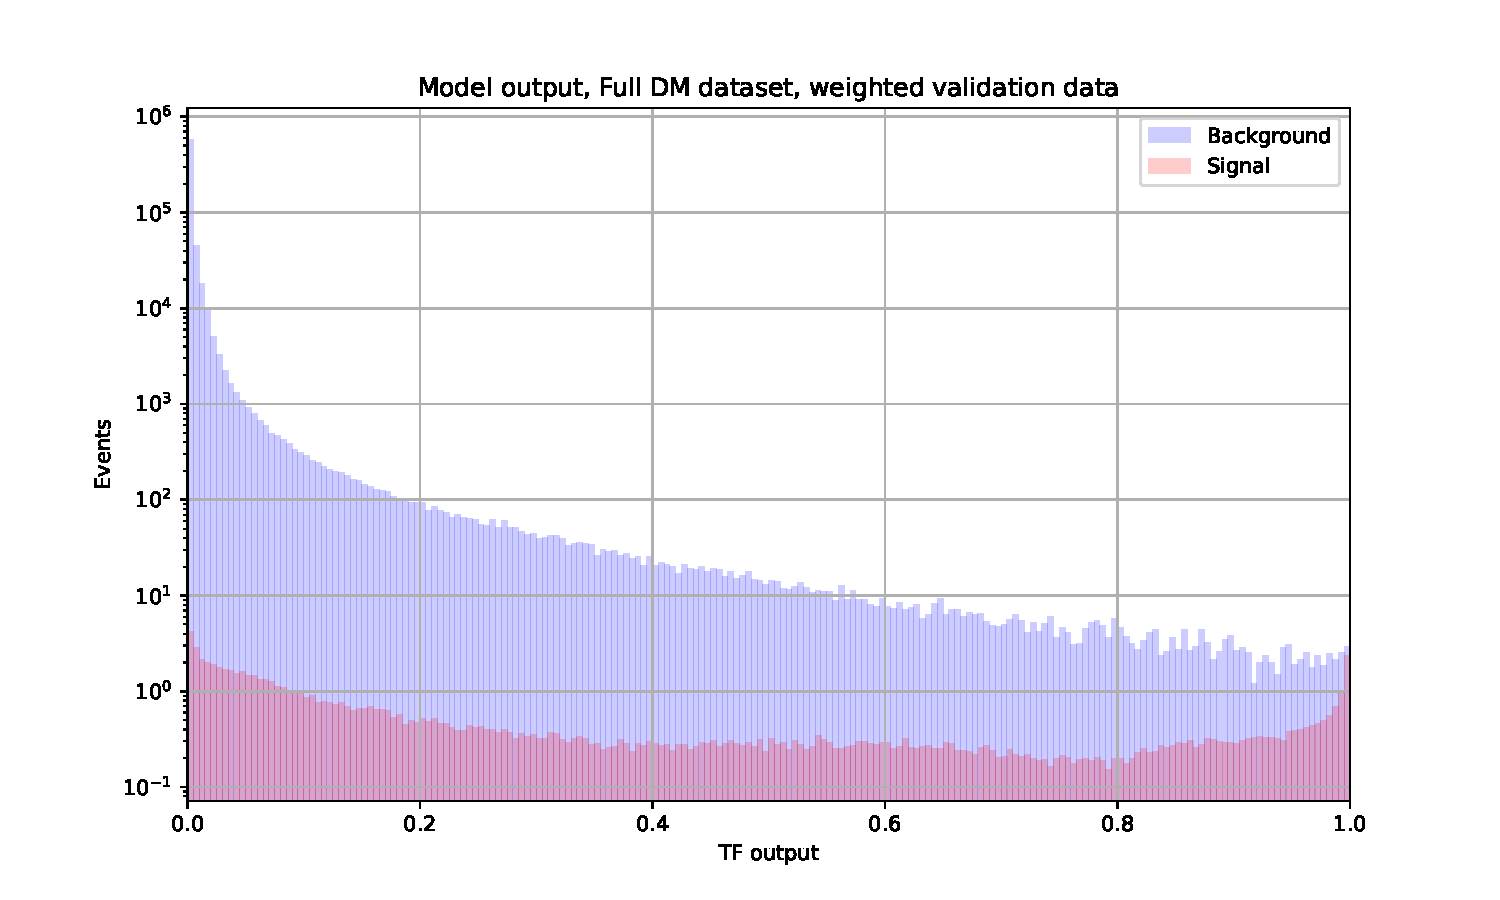
\includegraphics[width=1\textwidth]{OLD_DM_FULL_VAL_W.pdf}
        \caption{Scaled validation plot using MC weights.}\label{fig:OLD_W_FULL_DM_VAL}
     \end{subfigure}
	\caption{Validation plot of uwweighted network on the first version of the FULL DM dataset.}\label{fig:OLD_FULL_DM_VAL}
\end{figure}
\\\todo{The italics were my thoughts at the time}\textit{From my understanding it is preferable to train the network with weights, because then we can use it to predict data events, which have physical significance compared to MC events. This will be specially useful in my head when we predict how many dark matter events there are using real data, as this cannot be "scaled up" at a later point.}\\
\\\textit{As to which weights one shall use I am unsure, I like the physical weights for the reason above. But I know that for uneven datasets one could "weight down" the background events such that it "looks to be a 50-50 ratio" between background in signal. This sounds like making a bias in my head, and I would not know how to interpret the network predictions (if it predicts samples or events), but this appears to be a "standard" technique used in data science.}\\
\\T\textit{o check whether the network is working as intended I will now try to sort out "Diboson" events from other SM backgrounds, since we know this is real. If it works as intended I am unsure as to where to go next.} One thing worth noting is that the weights for the dark matter models being used may not necessarily be correct, as we don't have any empirical proof for the variables being used when calculating the weights (i.e. the cross section). \\
\\It seems that my interpretation was wrong, the weighted network for the Diboson search also predicted "0 Diboson events" (meaning my interpretation of the network predicting number of events is wrong), something we can empirically say is wrong (i.e. literally every figure of the kinematic variables). The scaled validation plot of the unweighted signal still "shows" that the network struggles a bit to see the difference between signal and background, overlapping almost all the way to 0.8. However it is still capable of sorting it out. Now I will try the "data analysts" way to weight the samples. That means weighting all background samples by $\frac{N_{sig}}{N_{bkg}}$, as is a common practice of weighting unbalanced datasets in data analysis.\\
\\The new weighting works! This is the method that will be used in the further studies using NNs. The \textit{Validation plots} showing the results of the network when trying to sort out the "Diboson" channel from the other are shown in Figure \ref{fig:DibosonVAL} and the ROC scores in Figure \ref{fig:DibosonROC}. A table showing how unbalanced the data is is showcased in Table \ref{tab:UnbalancedDibosonTraining}.\\
\begin{figure}[!ht]
	\centering
	\begin{subfigure}[b]{0.8\textwidth}
        \centering
        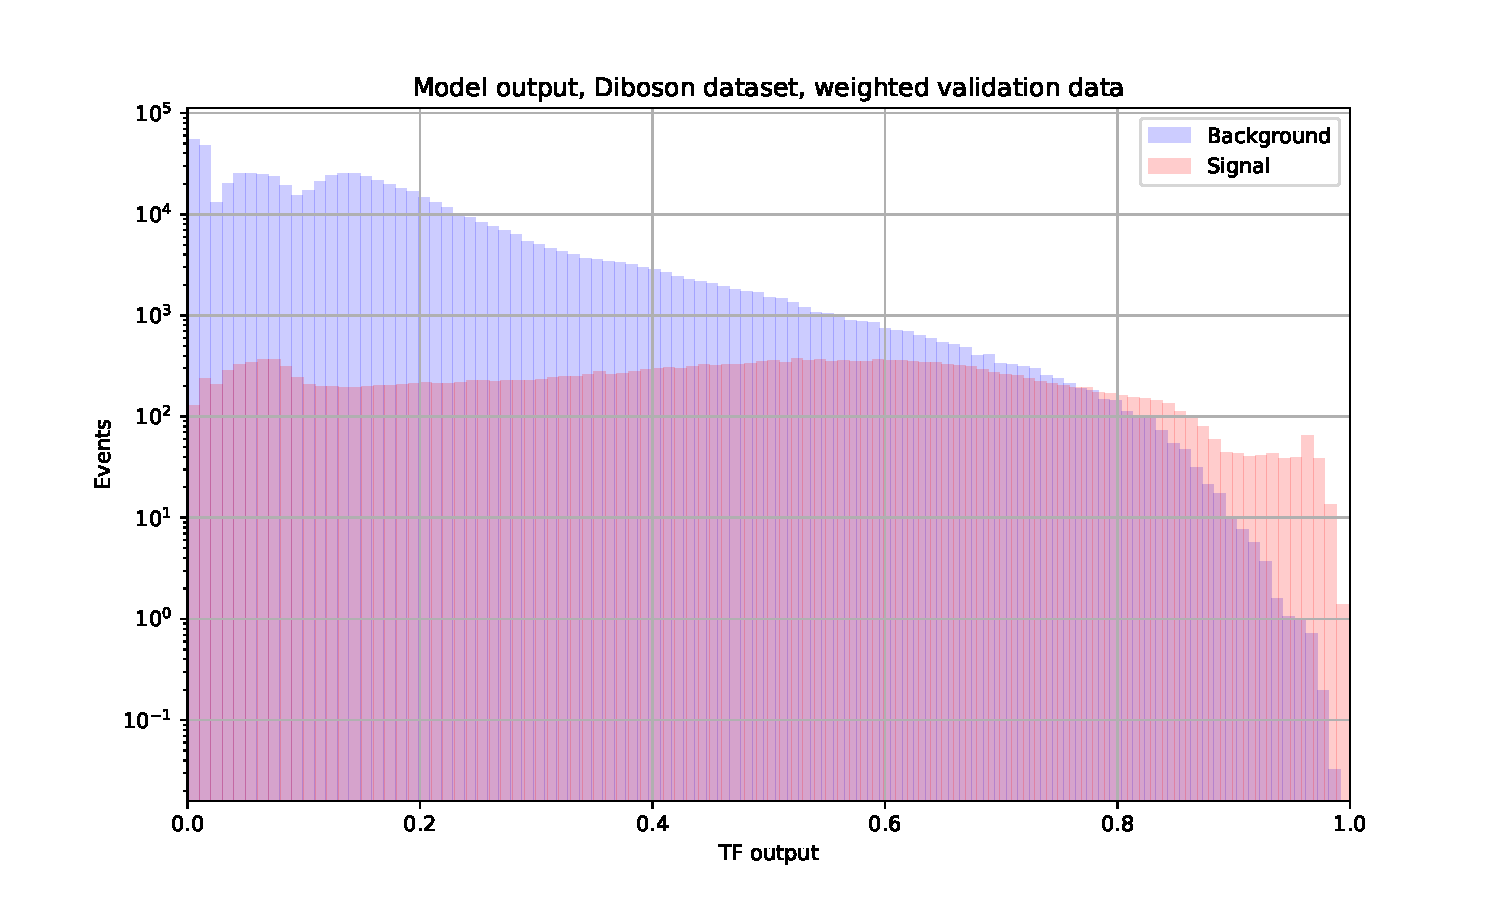
\includegraphics[width=1\textwidth]{VAL_uw.pdf}
        \caption{Validation plot for the unweighted training.}\label{fig:DibosonVALUW}
     \end{subfigure}
     \hfill
     \begin{subfigure}[b]{0.8\textwidth}
        \centering
        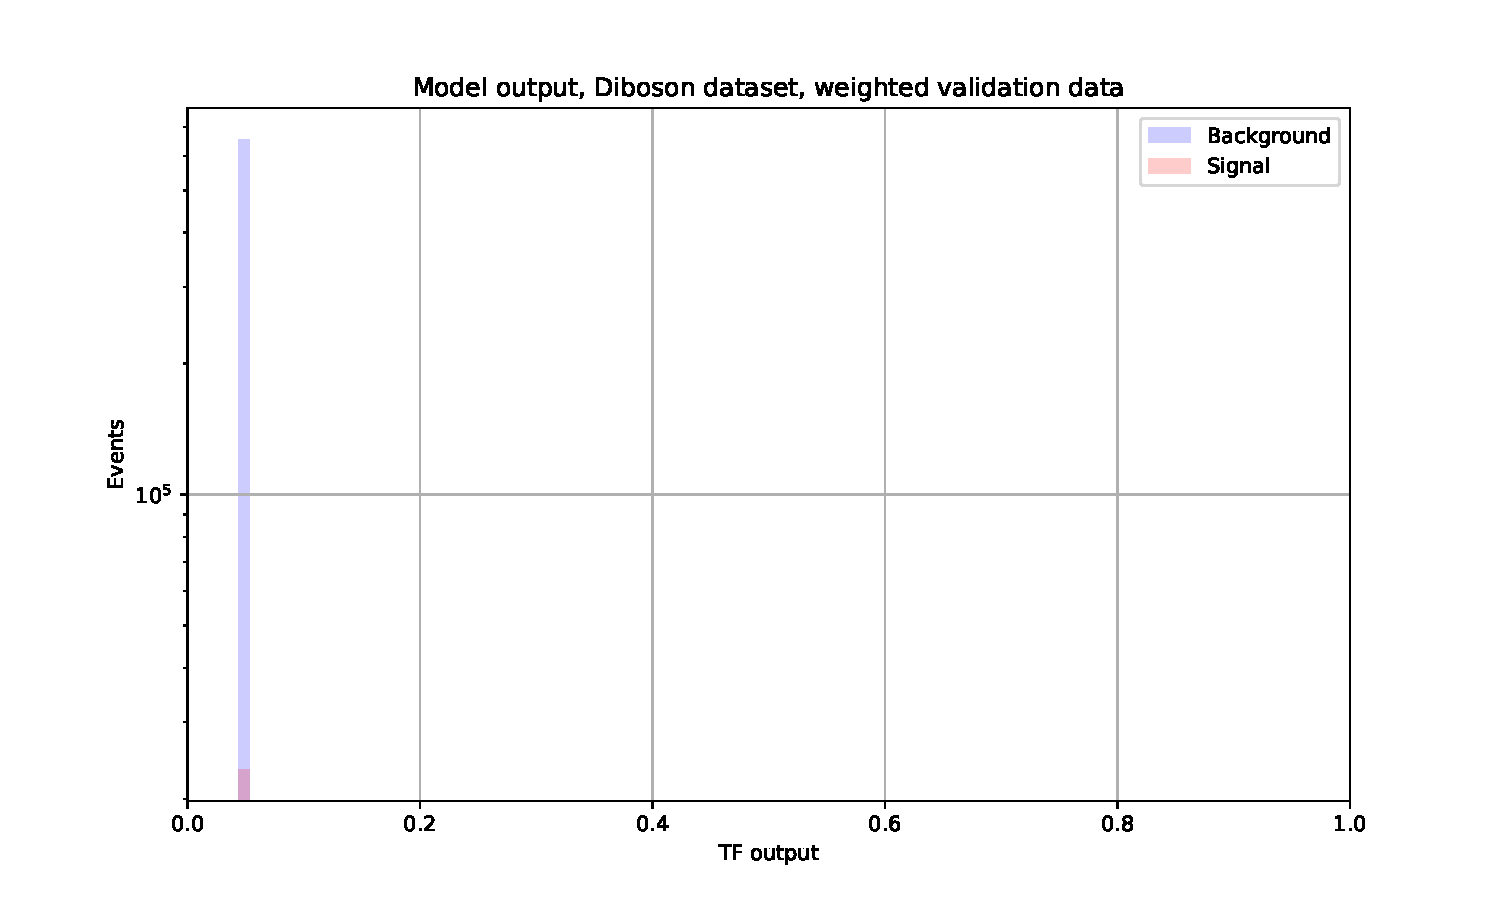
\includegraphics[width=1\textwidth]{VAL_mc.pdf}
        \caption{Validation plot for the weighted training using MC weights.}\label{fig:DibosonVALMC}
     \end{subfigure}
     \begin{subfigure}[b]{0.8\textwidth}
        \centering
        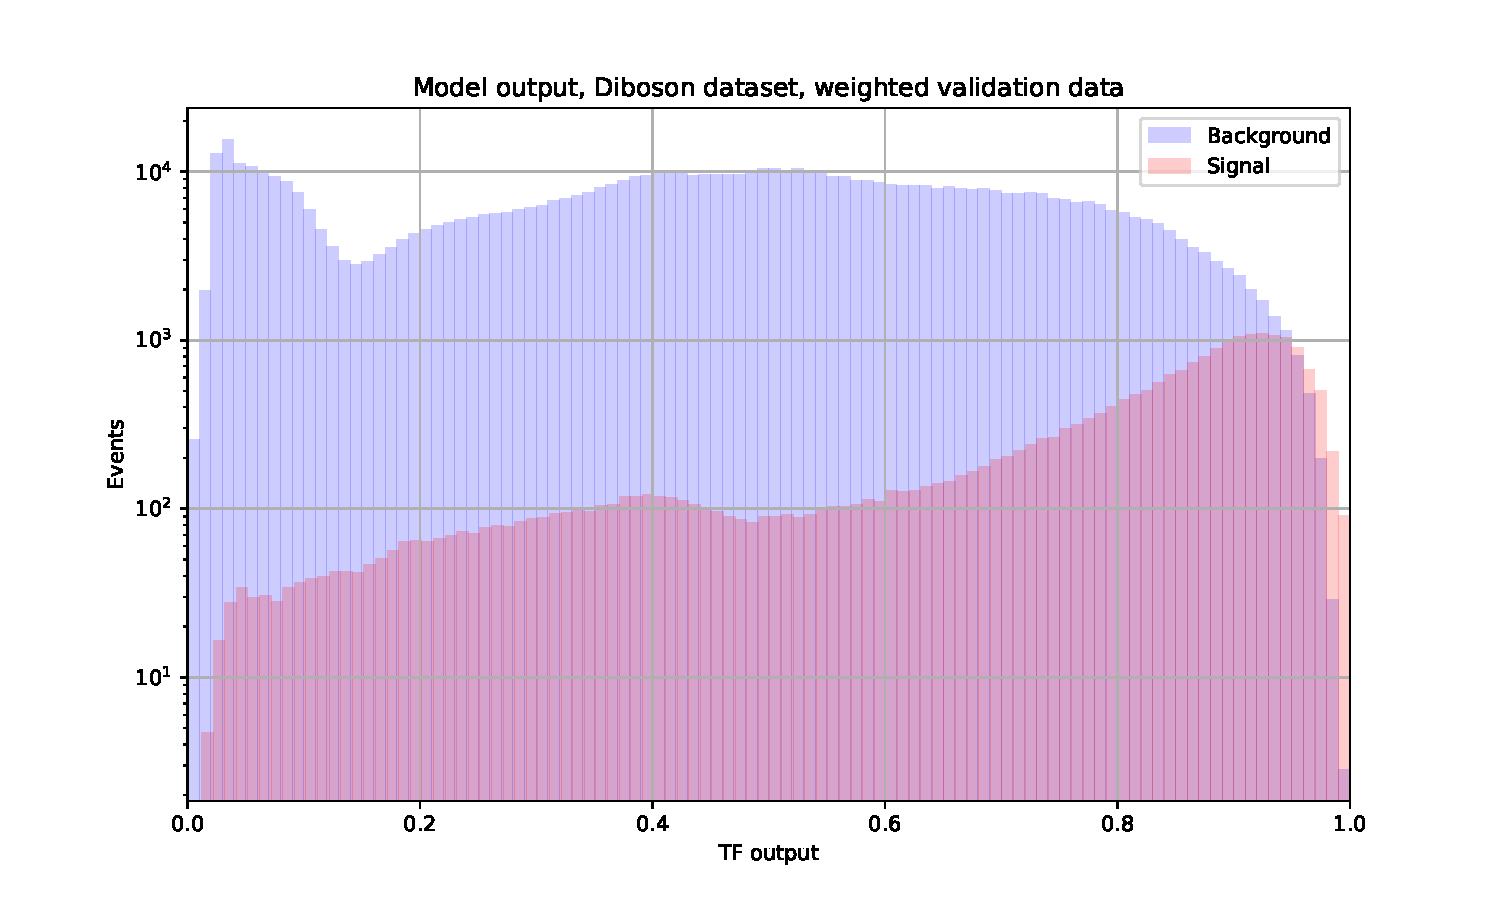
\includegraphics[width=1\textwidth]{VAL_w.pdf}
        \caption{Validation plot for the weighted training using $\frac{N_{sig}}{N_{bkg}}$ as weights on the background.}\label{fig:DibosonVALW}
     \end{subfigure}
	\caption{Result of the different network training weighting.}\label{fig:DibosonVAL}
\end{figure}
\begin{figure}[!ht]
	\centering
	\begin{subfigure}[b]{0.49\textwidth}
        \centering
        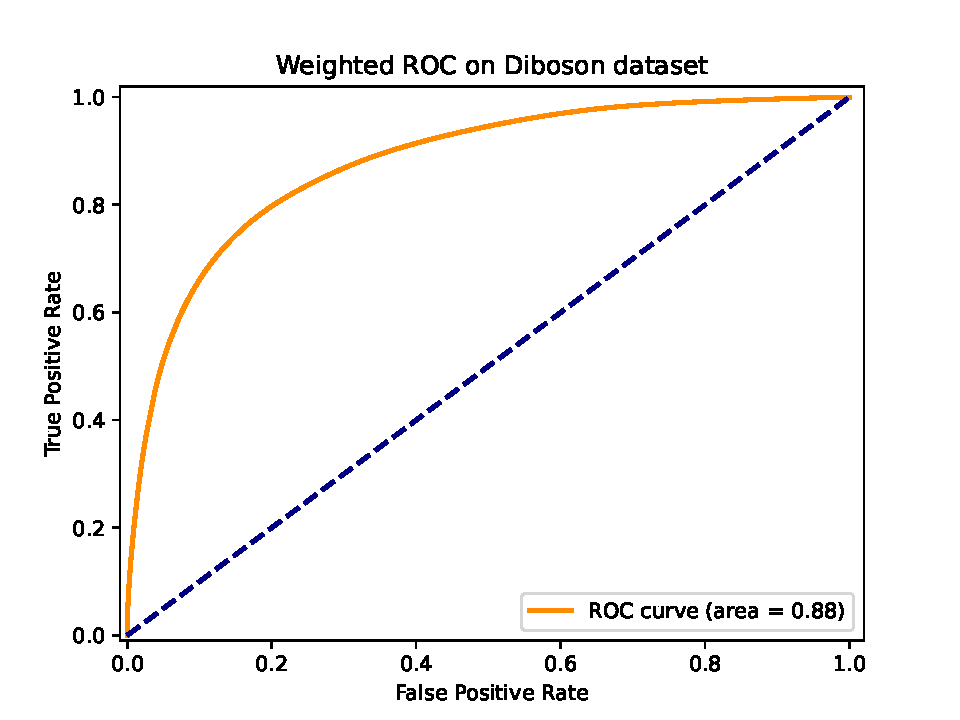
\includegraphics[width=1\textwidth]{ROC_uw.pdf}
        \caption{ROC score for the unweighted training.}\label{fig:DibosonROCUW}
     \end{subfigure}
     \hfill
     \begin{subfigure}[b]{0.49\textwidth}
        \centering
        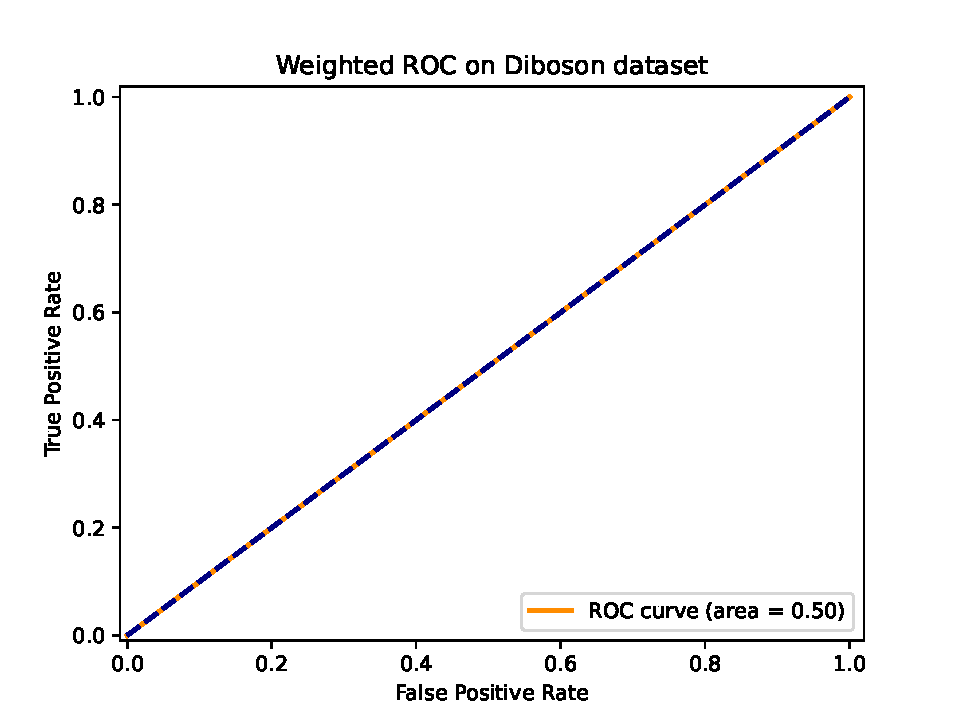
\includegraphics[width=1\textwidth]{ROC_mc.pdf}
        \caption{ROC score for the weighted training using MC weights.}\label{fig:DibosonROCMC}
     \end{subfigure}
     \begin{subfigure}[b]{0.49\textwidth}
        \centering
        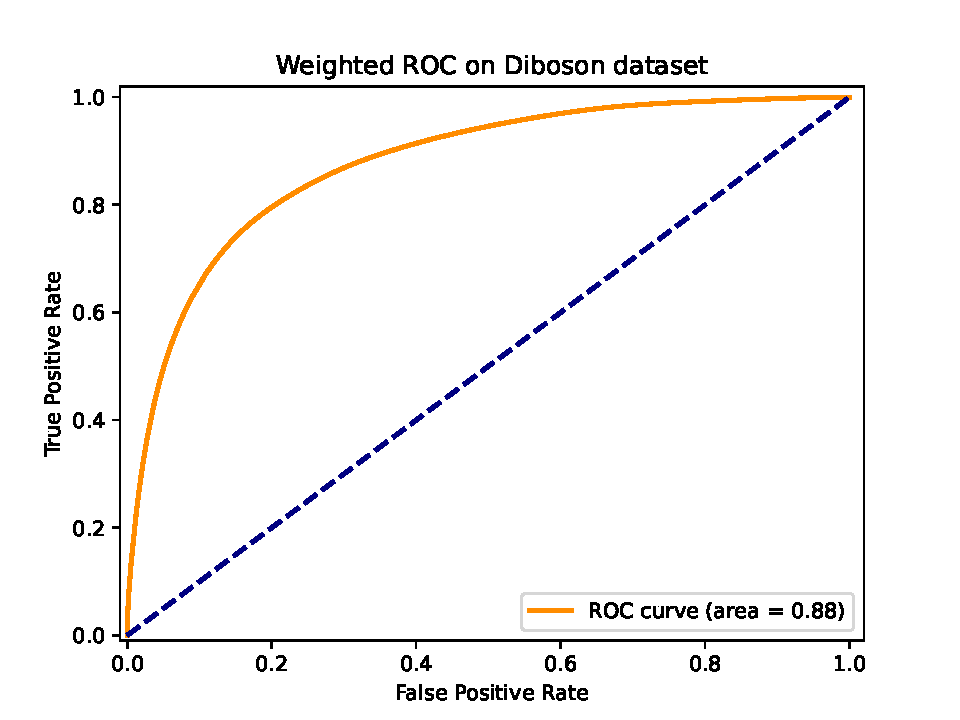
\includegraphics[width=1\textwidth]{ROC_w.pdf}
        \caption{ROC score for the weighted training using $\frac{N_{sig}}{N_{bkg}}$ as weights on the background.}\label{fig:DibosonROCW}
     \end{subfigure}
	\caption{Result of the different network training weighting.}\label{fig:DibosonROC}
\end{figure}
\begin{table}[!h]
    \centering
    \begin{tabular}{l|r|r|r}\midrule\midrule
                    & Number of events & Sum of weights & Events $\times$ SOW [$10^{11}$]\\\midrule
         Signal     & 8,813,716        & 93,304.9       & 8.2\\
         Background & 61,201,010       & 2,621,498.9    & 1,604.4 \\ \midrule\midrule
    \end{tabular}
    \caption[Unbalanced Diboson training dataset]{Table Showcasing how uneven the training dataset is between signal and background. This is on the Diboson dataset which incorporates all the SM MC samples}
    \label{tab:UnbalancedDibosonTraining}
\end{table}

\subsection{Balanced weights}
real events (SOW): bkg sig 2715280.423627234 388.36308153506815 
mc events (raw) 69664290 2991598
\clearpage


\section{XGBoost Training}
For XGBoost there is a different problem when it comes to weights. XGBoost has a variable called \verb|scale_pos_weight| where we can help the network deal with unbalanced data, such as the one we have. Thus we can use the \textit{real} weights that are calculated in the MC generators, except not really, XGBoost does not have to possibility to include negative weights. In this project I have therefore used the absolute value of the weights when training. Other than that there are few complications. 

\section{Pure log}
Some problems that have happened is that I had previously made a Deep Neural Network, using three hidden layers. This is however not optimal as the DM statistics is non existent compared to the SM background. Another big problem I had was that I used small bacth sizes when training the Neural Networks. A batch being a portion of the data which is used when training. The reason we batch is to reduce computational power and divide the task of learning. I had a batch size of around 30,000 MC events pr batch. To remind ourselves of our data size, we have around 90,000,000 MC events, from which roughly 40,000 corresponds to a single DM MC DSID. So when batching we trained the network to recognize DM, when there most likely wasn't a single DM sample in the batch itself... this explain the abrupt end, and peak of backgrounds on the signal region seen in Fig. \ref{fig:NN_EXP_SIG:uu}. Thankfully, since I have the supercomputer \verb|hepp03| available I could increase the batch size to a massive amount such as $2^24$ which gives roughly 16 million MC events pr bacth. This is the highest the GPU of the supercomputer can handle!\\
\\With this fixed there was still a big problem, the expected significance of both NN's and XGB is at best half of what a very rough cut and count gives. As mentioned in section 5.1.2, we can split the data in different forms. While splitting it pr DSID works with one hidden layer now it doesn't make much physical sense to do it the way I'm currently doing it when looking at the Z' DM models, since the DM MC samples are splitted into $ee$ and $\mu\mu$ final states. However if we train the network on either final state we are removing the model independent part of the plan (although this increases the significance!). The plan fowards so far is to combine the final states of the Z' DM models as long as they only differ in final lepton state. And compare the significance of these to a statistically combined significance of cut and count.\\
\\One last thing to add as to why the significance might be so much lower for our networks is that I have not yet done a grid search for the best hyperparameters and loss functions. Doing this with XGBoost is easy, but there is a memory leak in the codebase of TensorFlow that makes the process tedious... This is where I am at in the present time, as well as waiting for more DM data.

\section{Comparison to cut and count}
Testing three models using the classical data analysis way we apply cuts to kinematic variables and try to isolate the signal from the background to then calculated the expected significance. The three models I chose to test are all High Dark Sector models with $m_{Z'}=130$GeV. They are a Light Vector (LV), Dark Higgs (DH) and Effective Field Theory (EFT) models. The cuts I made on these are shown in Table \ref{tab:cuts}.
\begin{table}[!h]
    \centering
    \begin{tabular}{l|r}\midrule\midrule
                                & Cut\\\midrule
         $E_T^{miss}/\sigma$    & > 10      \\
         $m_T$                  & > 160 GeV \\
         $m_{ll}$               & > 120 GeV \\
         Number of B-jets       & 0         \\
         $m_{T2}$               & > 110 GeV \\\midrule\midrule
    \end{tabular}
    \caption[Cut and count cuts]{Table showcasing the cuts used when doing the cut and count method.}
    \label{tab:cuts}
\end{table}
\\ Since the cross section to find Dark Matter is really small we have to use the low-statistics expected significance formula to find the closest to correct significance. The formula is
\begin{equation}\label{eq:low_stat_Z}
    Z = \sqrt{2\left[(s + b)\ln(1 + \frac{s}{b}) - s \right]}
\end{equation}
Where $s$ is the number of signal events and $b$ is the number of background events. Using this we get the results shown in Table \ref{tab:cutsigee} for the electron channel and Table \ref{tab:cutsiguu} for the muon channel. Also included on the tables are the number of events. One thing worth mentioning is that when adding another cut on the maximum invariant mass increases the significance. The significance for LV on the electron channel was at $1.2\sigma$ when adding a cut stating that $m_{ll}<150$ GeV. This makes sense since the models in question all have a $m_{Z'}=130$GeV. This cut was not added since we do not want to put a cap on the mass of the propagator, as we don't know what the real mass is.
\begin{table}[!h]
    \centering
    \begin{tabular}{l|c|c|c|r}\midrule\midrule
                                          & LV  & DH  & EFT & Background \\\midrule
         Events before cuts               & 15  & 20  & 0   & 1,256,624    \\
         Events after cuts                & 4   & 6   & 0   & 117 \\
         Expected significance [$\sigma$] & 0.4 & 0.6 & 0   & \\\midrule\midrule
    \end{tabular}
    \caption[Cut and count significance ee]{Table showcasing the result of the cut and count method for the electron channel.}
    \label{tab:cutsigee}
\end{table}
\begin{table}[!h]
    \centering
    \begin{tabular}{l|c|c|c|r}\midrule\midrule
                                          & LV  & DH  & EFT & Background \\\midrule
         Events before cuts               & 14  & 19  & 0   & 1,626,098    \\
         Events after cuts                & 3   & 5   & 0   & 108 \\
         Expected significance [$\sigma$] & 0.36 & 0.51 & 0   & \\\midrule\midrule
    \end{tabular}
    \caption[Cut and count significance uu]{Table showcasing the result of the cut and count method for the muon channel.}
    \label{tab:cutsiguu}
\end{table}
\\If we were to compare these results with what our NN and BDT that trained on the full dataset we see that we can calculate the expected significance in different locations for the validation plots. Testing on the networks that trained using the data scientist method on the full DM dataset we get the results shown in Figure \ref{fig:XGB_SIG_FULL} for XGBoost and Figure \ref{fig:NN_SIG_FULL} for the Neural Network.
\begin{figure}[!ht]
	\centering
	\begin{subfigure}[b]{0.8\textwidth}
        \centering
        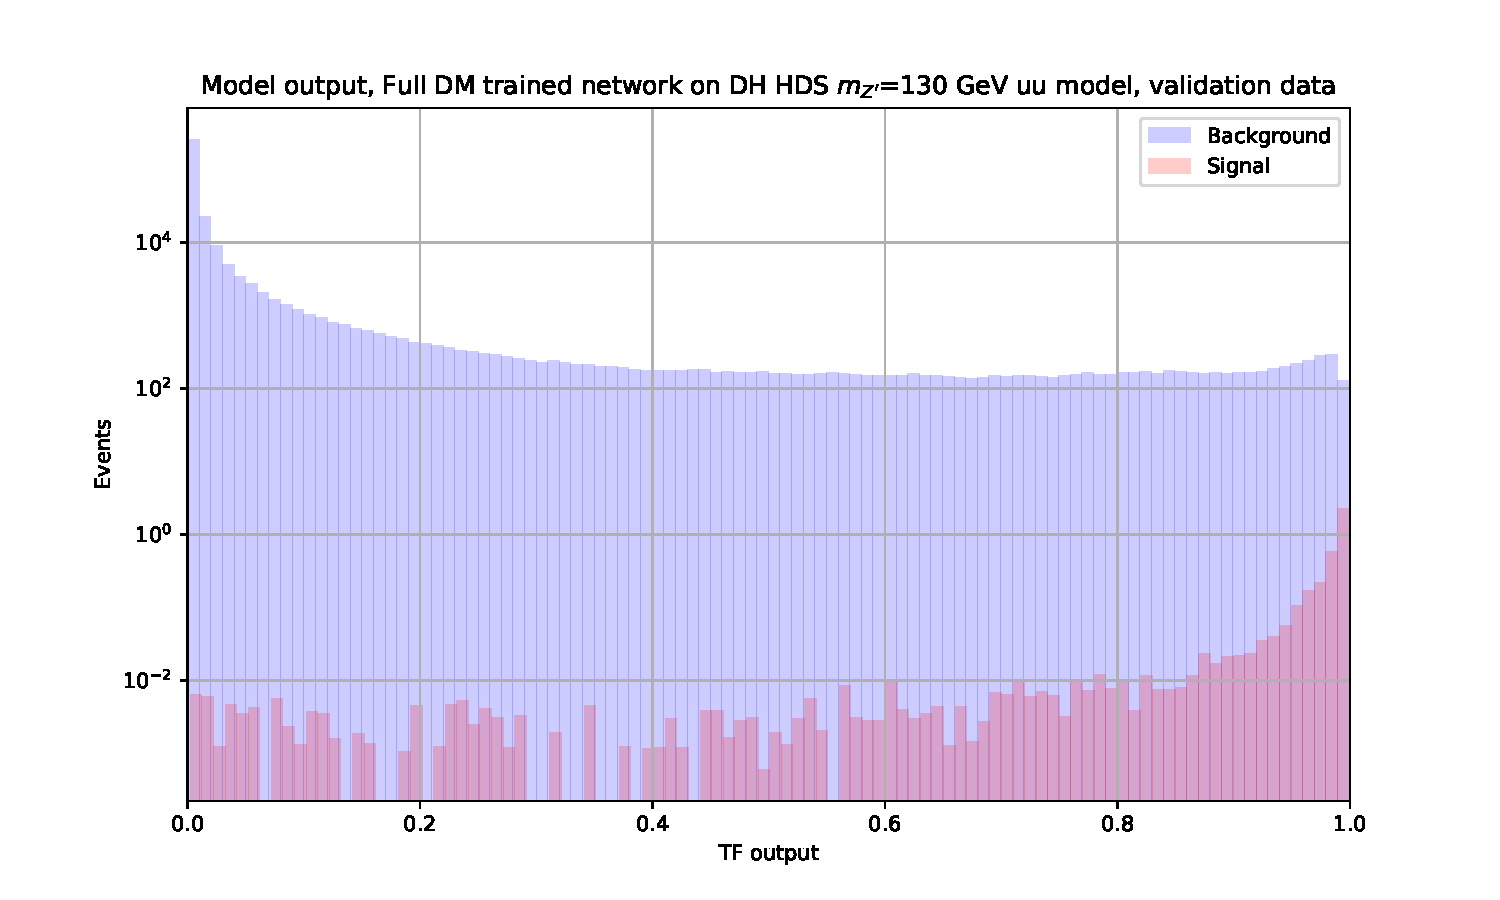
\includegraphics[width=1\textwidth]{XGB_VAL_uu.pdf}
        \caption{Validation plot.}\label{fig:XGB_VAL_UU}
     \end{subfigure}
     \hfill
     \begin{subfigure}[b]{0.8\textwidth}
        \centering
        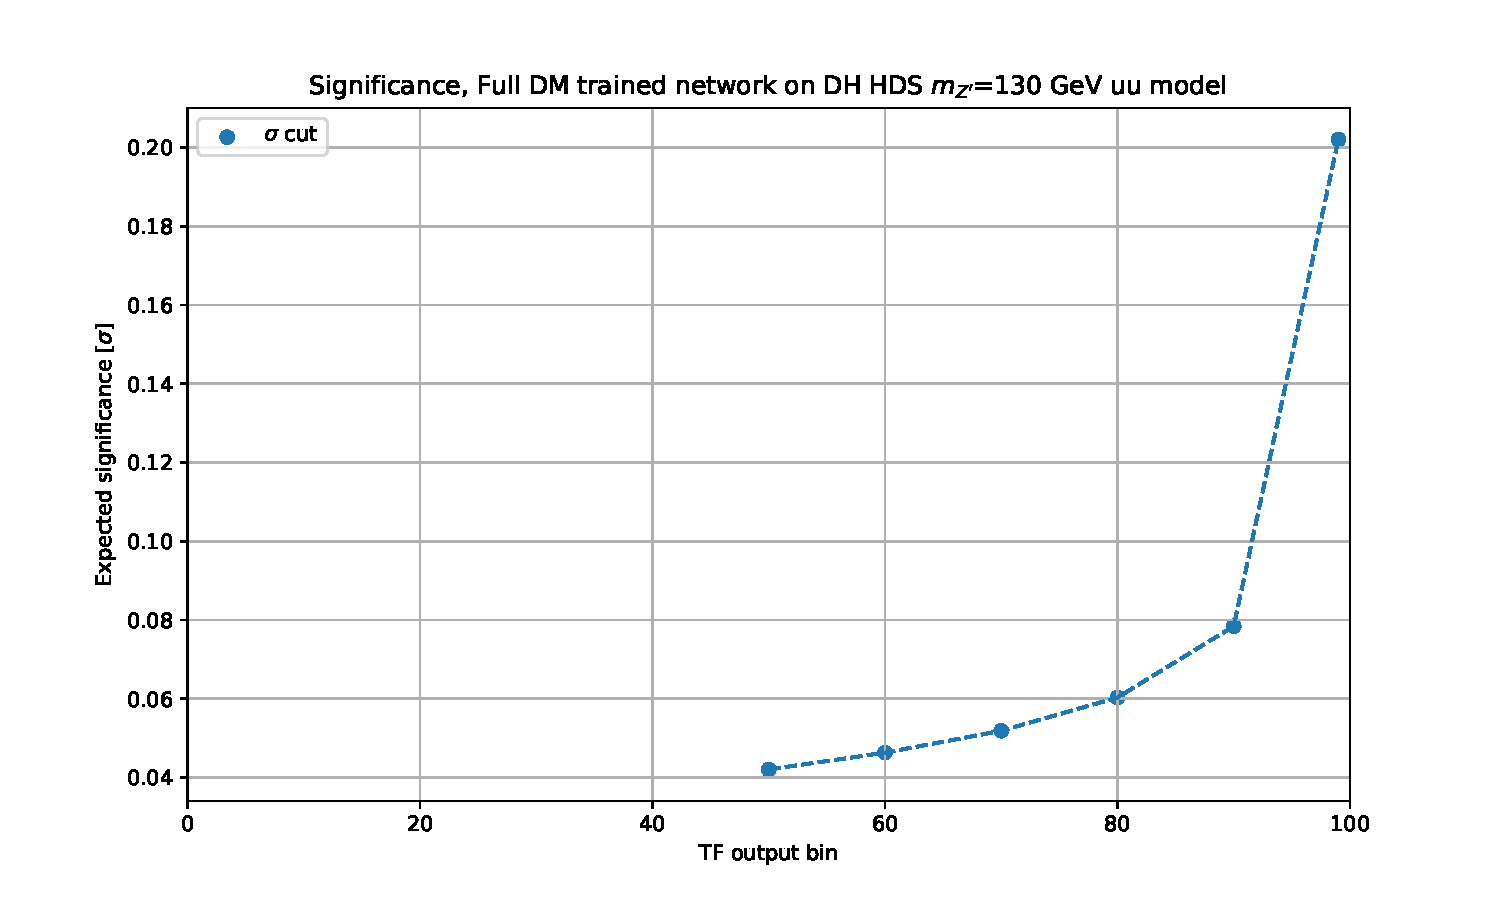
\includegraphics[width=1\textwidth]{XGB_EXP_SIG_uu.pdf}
        \caption{Expected significance when looking at bins and forth.}\label{fig:XGB_EXP_SIG:uu}
     \end{subfigure}
	\caption{Expected significance of XGBoost when trained on the Full DM dataset for the DH HDS $m_{Z'}$ = 130 GeV muon model.}\label{fig:XGB_SIG_FULL}
\end{figure}
\begin{figure}[!ht]
	\centering
	\begin{subfigure}[b]{0.8\textwidth}
        \centering
        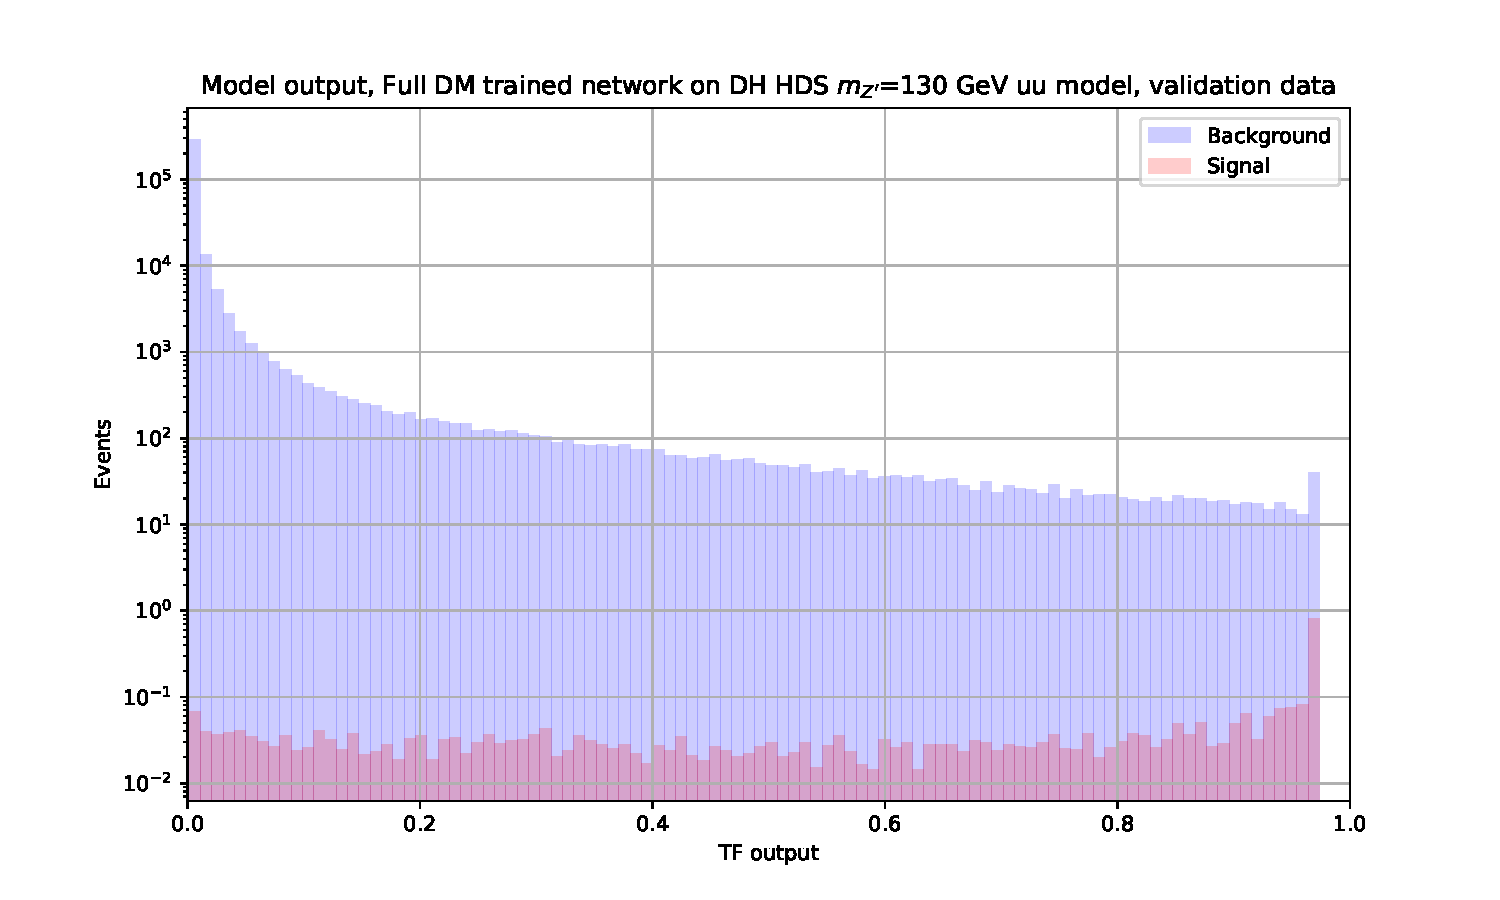
\includegraphics[width=1\textwidth]{NN_VAL_uu.pdf}
        \caption{Validation plot.}\label{fig:NN_VAL_UU}
     \end{subfigure}
     \hfill
     \begin{subfigure}[b]{0.8\textwidth}
        \centering
        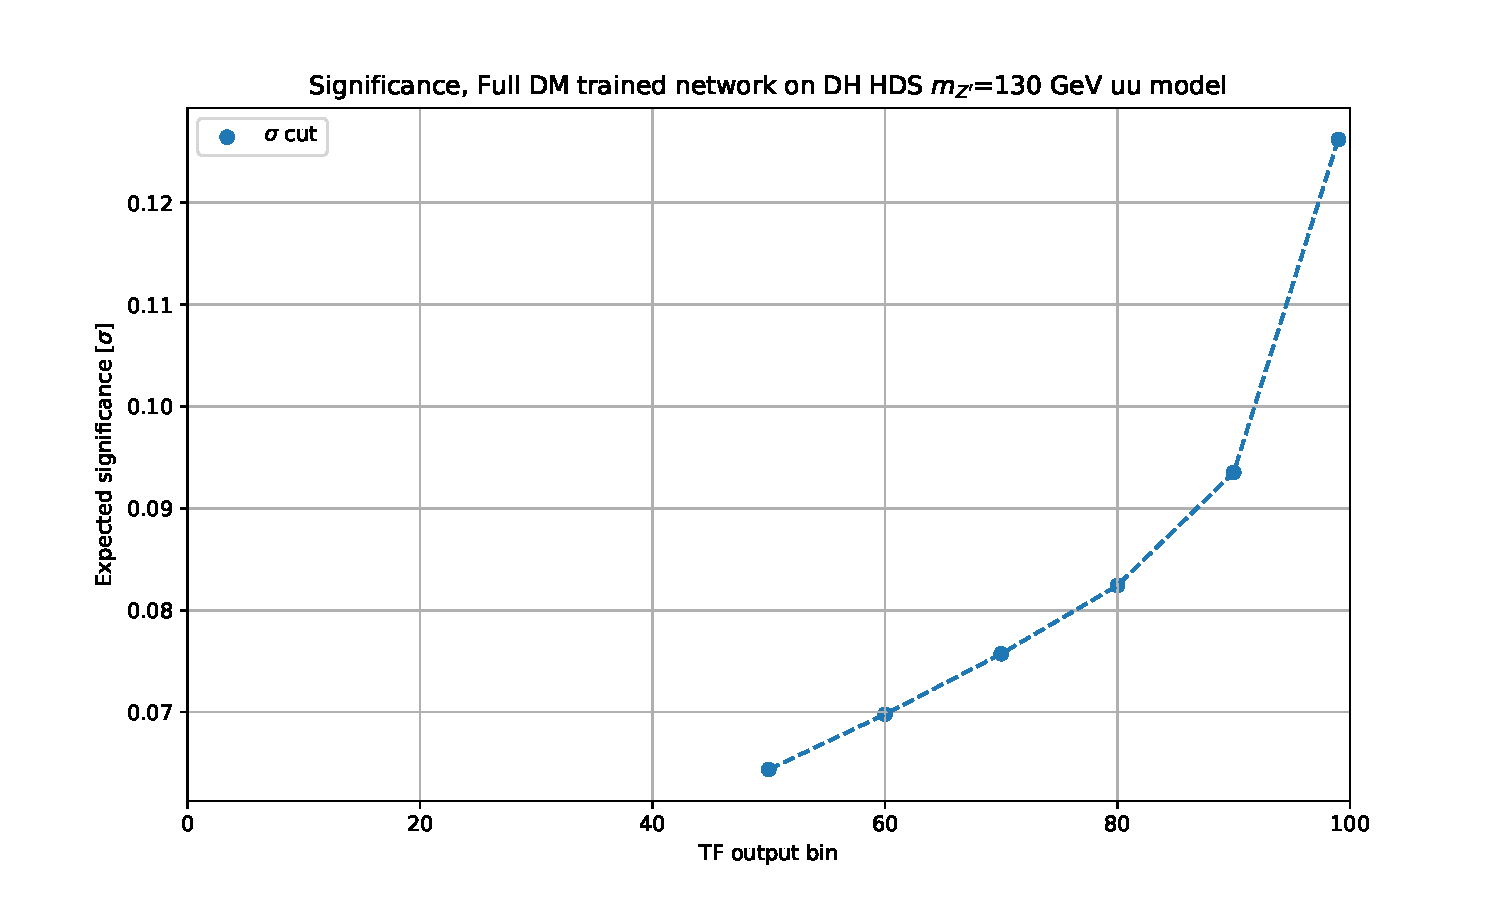
\includegraphics[width=1\textwidth]{NN_EXP_SIG_uu.pdf}
        \caption{Expected significance when looking at bins and forth.}\label{fig:NN_EXP_SIG:uu}
     \end{subfigure}
	\caption{Expected significance of the Neural Network when trained on the Full DM dataset for the DH HDS $m_{Z'}$ = 130 GeV muon model.}\label{fig:NN_SIG_FULL}
\end{figure}
\clearpage As we can see the expected significance is lower using ML than a rough cut and count. My theory for why this is the case is because we are testing just \textit{\textbf{one}} sample out of 154 different ones that are included for the three different theories I have acquired so far. And the ML networks shown above have both trained on a dataset including all 154 DM samples. The models that I tested might also not have been one of the "important" models the network learned from. Thus if I were to train the network individually based on the theory it might give better results.


\part{Results}

\begin{table}[!h]
    \centering
    \begin{tabular}{l|c|c|c}\midrule\midrule
                    & Number of events & Sum of weights & Events $\times$ SOW [$10^{13}$]\\\midrule
         Signal     & 2,991,543        & 36,327,943.99  & 1.08\\
         Background & 69,664,345       & 36,327,944.03  & 25.3 \\ \midrule\midrule
    \end{tabular}
    \caption[Unbalanced DM training dataset]{Table Showcasing how uneven the training dataset is between signal and background. This is on the dataset which incorporates all the different DM MC samples}
    \label{tab:UnbalancedDMTraining}
\end{table}
in spacetime.

%\printbibliography

\end{document}
